\chapter[Algoritmo Proposto]{Algoritmo Proposto}

O algoritmo proposto para a solução descrita neste sistema baseia-se em uma técnica clássica de super-resolução \cite{garcia2013tecnicas}. O termo super-resolução (SR) é usado para descrever processos que procuram acrescentar informações de alta frequência a uma imagem interpolada a partir de uma ou mais imagens disponíveis \cite{baker2002limits,park2003super,farsiu2004advances}. Este conjunto de imagens pode ser formado por imagens decimadas ou adquiridas por múltiplos sensores capturando uma mesma cena durante determinado período de tempo. Para cenas estáticas (Figuras \ref{fig:SR_1} e \ref{fig:SR_2}), as observações são relacionadas por deslocamentos globais em nível de \textit{subpixel}, geralmente ocorrendo devido a posições relativas das câmeras ou movimento do próprio sensor. Para cenas dinâmicas, as observações são relacionadas a deslocamentos de \textit{subpixel} devidos ao movimento local dos próprios objetos juntamente com os deslocamentos globais, conforme pode ser visualizado na Figura \ref{fig:SR_3}. Em ambos os casos, a super-resolução é utilizada para gerar uma imagem com maior resolução espacial a partir de um conjunto de imagens em baixa resolução ou de frames de uma sequência de vídeo \cite{figueira2013super}\cite{milanfar2010super}.
\\

\begin{figure}[h]
    \centering
    \subfloat[]{
	    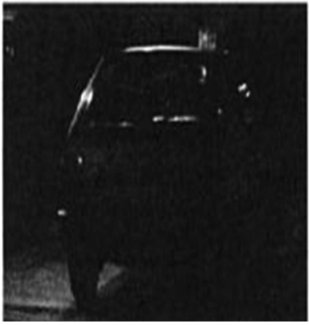
\includegraphics[width=0.4\linewidth]{figuras/SR_img_1a.png}\label{fig:SR_1a}
    }
    \qquad
    \subfloat[]{
    	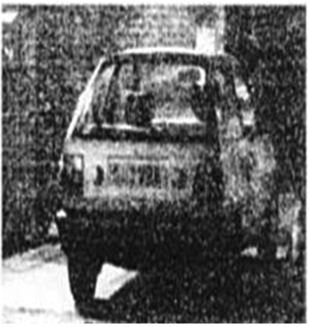
\includegraphics[width=0.4\linewidth]{figuras/SR_img_1b.png}\label{fig:SR_1b}
    }
    \caption{(a) uma cena estática de uma sequência de vídeo é capturada com baixa luminosidade; (b) após equalização de histograma a placa do automóvel continua ilegível devido ao ruído natural da imagem. Fonte: \cite{kang2000digital}. }%
	    \label{fig:SR_1}
\end{figure}

\clearpage
\begin{figure}[h]
	\centering
	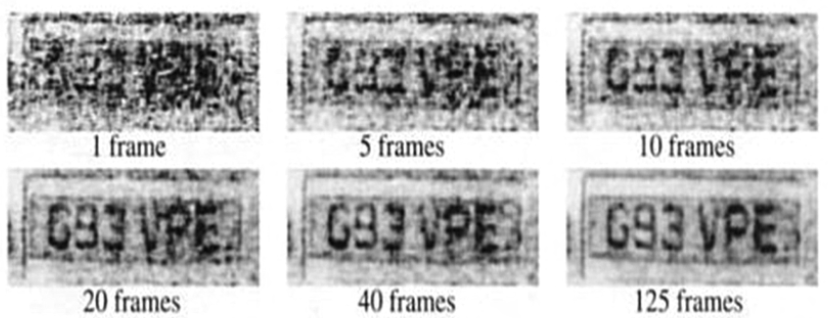
\includegraphics[scale=0.45]{figuras/SR_img_2.png}
	\caption{Legibilidade da placa como resultado da média do conjunto cada vez maior de quadros. Fonte: \cite{kang2000digital}.} 
	\label{fig:SR_2}
\end{figure}

\begin{figure}[h]
    \centering
    \subfloat[]{
	    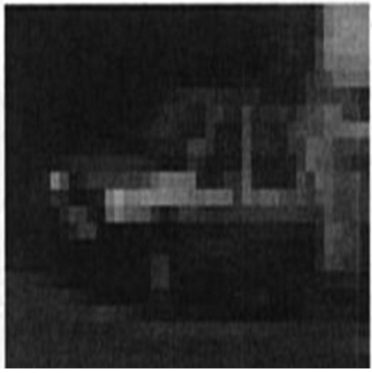
\includegraphics[width=0.4\linewidth]{figuras/img_SR_3a.png}\label{fig:SR_1a}
    }
    \qquad
    \subfloat[]{
    	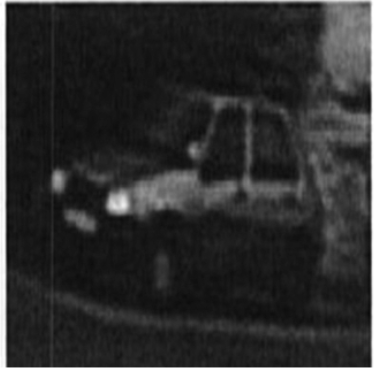
\includegraphics[width=0.4\linewidth]{figuras/img_SR_3b.png}\label{fig:SR_1b}
    }
    \caption{(a)  região de interesse é capturada em uma cena dinâmica; (b) a SR estima a cena subjacente a partir de 50 imagens. A reconstrução possui o triplo da resolução em relação à imagem original. Fonte: \cite{kang2000digital}. }%
	    \label{fig:SR_3}
\end{figure}

    Presupõe-se que a simples interpolação dessas imagens não seja suficiente para representar a cena de interesse com nitidez, fazendo-se necessário processar e combinar as diversas imagens disponíveis. É possível que todas as imagens possuam a mesma resolução, de forma que a super-resolução seja através da combinação dessas imagens (super-resolução por combinação de múltiplas imagens), ou que a imagem de interesse em baixa resolução seja processada a partir de um banco de imagens em alta resolução (super-resolução por exemplos) \cite{garcia2013tecnicas}. Neste trabalho trataremos apenas do segundo tipo de super-resolução.


\section{Super-resolução por exemplos}
\label{SR_exemp}
A técnica de super-resolução baseada em exemplos busca informações de alta frequência em uma base de dados com imagens em alta resolução para adicioná-los a uma imagem interpolada. A princípio, não há relação direta entre a base de dados e a imagem de entrada, de forma que o algoritmo pode atender a uma ampla gama de imagens em baixa resolução, com um grande banco de dados \cite{freeman2002example}. Esta técnica baseia-se no fato que a coleção de imagens que capturam cenas reais, por exemplo, possui variabilidade muito menor do que a coleção de imagens aleatórias \cite{garcia2013tecnicas}.

Na super-resolução baseada em exemplos, gera-se para cada imagem em alta resolução $I_j$ uma versão com componentes de baixa frequência, $I_j^B$, e uma versão de componentes de alta frequência, $I_j^A$, onde $I_j^A$ = $I_j$ - $I_j^B$. Assim considera-se a imagem interpolada $I_0$ correspondente somente as componentes de baixa frequência ($I_0 = I_0^B$ ), o que permite obter uma relação entre a imagem de entrada ($I_0$) e as imagens de referência ($I_j$) \cite{garcia2013tecnicas}.

$I_0^B, I_j^B$ e $I_0^A$ são divididas em blocos regulares, e procura-se em $I^B_j$ pelo bloco mais semelhante a cada um dos blocos de $I_0^B$. De acordo com a posição do bloco escolhido em $I_j^B$, extrai-se o bloco em $I_j^A$. Este bloco de alta frequência é então somado a $I_0$, acrescentando detalhes que foram perdidos após da decimação. Tal processo é ilustrado na Figura \ref{fig:SR_4}.

\begin{figure}[h]
	\centering
	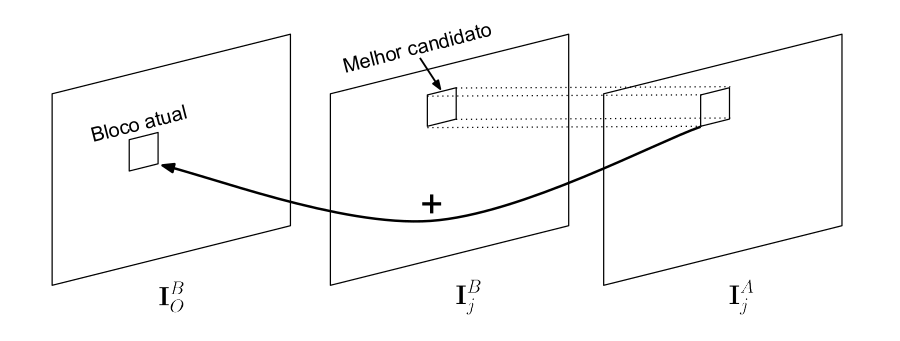
\includegraphics[scale=0.50]{figuras/superresolucao_4.png}
	\caption{Super-resolução baseada em exemplos: a imagem interpolada $I_0^B$ recebe informações de alta frequência a partir de uma imagem em alta resolução $I_j$ separada em versões com componentes de baixa e alta frequência, $I_j^B$ e $I_j^A$. Fonte: \cite{garcia2013tecnicas}.}

	\label{fig:SR_4}
\end{figure}

\section{Solução proposta}

Devido a pequena largura de banda disponível para o envio dos dados, optou-se por enviar uma sequência de vídeo com quadros em resolução mista, como ilustrado pela Figura \ref{fig:resolucao_mista}. 

\begin{figure}[h]
	\centering
	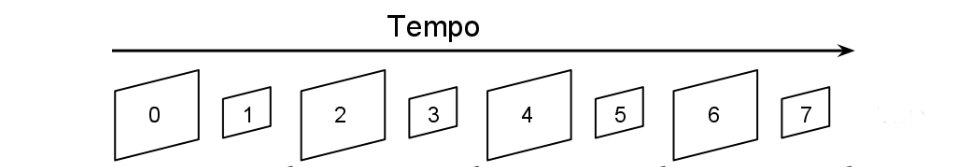
\includegraphics[scale=0.45]{figuras/resolucao_mista.png}
	\caption{ Arquitetura de codificação em resolução mista.}

	\label{fig:resolucao_mista}
\end{figure}

A fim de recuperar as informações de baixa frequência dos quadros em baixa resolução, apresenta-se uma técnica baseada na super-resolução por exemplos. Assim, utiliza-se como banco de dados as imagens adjacentes ao quadro que será super-resolvido, que possuem alta correlação que com o mesmo.

O fluxograma mostrado na Figura \ref{fig:algoritmo_proposto}, ilustra do algoritmo proposto. Dado um quadro original  decimado ($I_O^D$),  para ficar em baixa resolução, ele é interpolado à sua resolução original,  gerando $I_O^B$, este por usa vez constitui uma versão de baixa frequências do quadro original $I_O$. O objetivo final do algoritmo proposto é gerar uma versão super-resolvida  $I_O chapeu$ mais semelhante ao quadro original, a partir das estimativas $\widehat{I}_A$ de alta frequência $I_O^A$. Aqui, assume-se que:

\begin{equation}
\widehat{I}_0 = I_O^B + \widehat{I}_O^A.
\label{eq_HF}
\end{equation}

\begin{figure}[h]
	\centering
	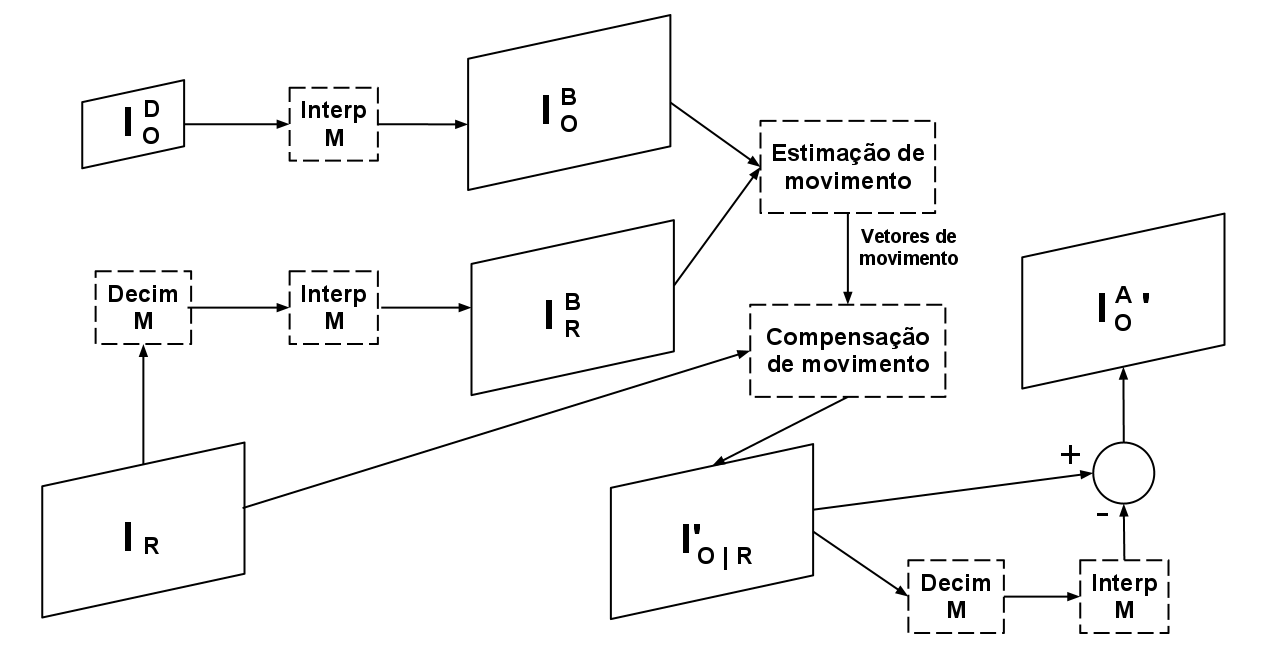
\includegraphics[scale=0.30]{figuras/fluxo_super_resolucao.png}
	\caption{Fluxograma do algoritmo de super-resolução proposta.}
	\label{fig:algoritmo_proposto}
\end{figure}

Definindo $I_R$ como o quadro adjacente é gerada sua versão de baixa frequências $I_R^B$, por um processo de decimação seguido de uma interpolação utilizando o mesmo fator $M$ que foi utilizado em $I_O$ em seguida aplica-se o processo de busca pelos blocos semelhantes descrita na Seção \ref{SR_exemp}, também chamado de estimação de movimento, entre $I_O^B$ e $I_R^B$. Assim para cada bloco $(u_i,v_i)$, obtêm-se vetores de movimento $(m_u,m_v)$ que representam a posição do bloco mais parecido com o procurado. 

    De posse desses vetores de movimento, gera-se a estimativa de alta frequência de $I_O$, realizando a compensação de movimento, que consistem em reorganizar os blocos da imagem de acordo com os vetores de movimento, na versão de altas frequências da imagem de referência ($I_R^{A}$) obtida de acordo com a equação Zeta, ou seja, $I_R^{A} = I_R - I_R^B$. Assim para cada bloco $(u_i,v_i)$, têm-se:

\begin{equation}
I_R^{A’} (u_i,v_i) = I_R^A(u_i+m_u, v_i+m_v).
\end{equation}


O quadro $I_R^{A’} $ já pode ser considerado uma estimativa de alta frequência de $I_O$. Ele busca correlação entre os blocos de baixa frequência $I_0^B$ e $I_R^B$, assumindo que as altas frequências de $I_R$ são uma boa estimativa para $I_O^A$. Restando assim, somar as componentes de baixa frequência com as de alta para ter a estimativa de $Î_O$.